\chapter{Anorganische materialen en nanomaterialen}\label{ch:b3:inorganic-materials}

Een plaat \omterm{def:b3:inorganic-materials:sol-gel}{silica-aerogel}, een vaste stof die grotendeels uit lucht
bestaat, houdt een bloem boven een gasvlam zonder dat ze verwelkt. Het is
een glas, niet gemaakt door zand te smelten, maar door een vloeistof tot
een \omterm{def:b3:colloids:colloid}{gel} te laten opstijven en die \omterm{def:b3:colloids:colloid}{gel} daarna te drogen zonder dat hij
inzakt. De materiaalchemie werkt in die volgorde: kies de structuur, dan
de route die haar maakt, en lees daarna de eigenschappen af. Dit
hoofdstuk volgt de routes naar anorganische vaste stoffen, de structuren
van \omterm{def:b3:inorganic-materials:ceramic}{keramiek}, glazen en poreuze kristallen, en wat er met materie
gebeurt als een deeltje maar enkele nanometer groot is.

\begin{recall}
Het deel van jaar~1 beschreef structuurtypen van kristallen,
interstitiële holten, allotropen, grafiet en diamant; het deel van jaar~2
fasediagrammen, de glasovergangstemperatuur en polymeren.
\Cref{ch:b3:surfaces-catalysis} definieerde het
\omterm{def:b3:surfaces-catalysis:surface-area}{specifiek oppervlak}, \cref{ch:b3:colloids} \omterm{def:b3:colloids:colloid}{solen} en \omterm{def:b3:colloids:colloid}{gels},
\cref{ch:b3:solid-state} banden, \omterm{def:b3:solid-state:defects}{puntdefecten} en \omterm{def:b3:solid-state:ionic-conductor}{ionengeleiders};
\cref{ch:b3:quantum-model-systems} loste het \omterm{def:b3:quantum-model-systems:box}{deeltje in een doos} op, en
\cref{ch:b3:point-groups} gaf de icosaëdrische groep.
\end{recall}

\begin{omfigure}
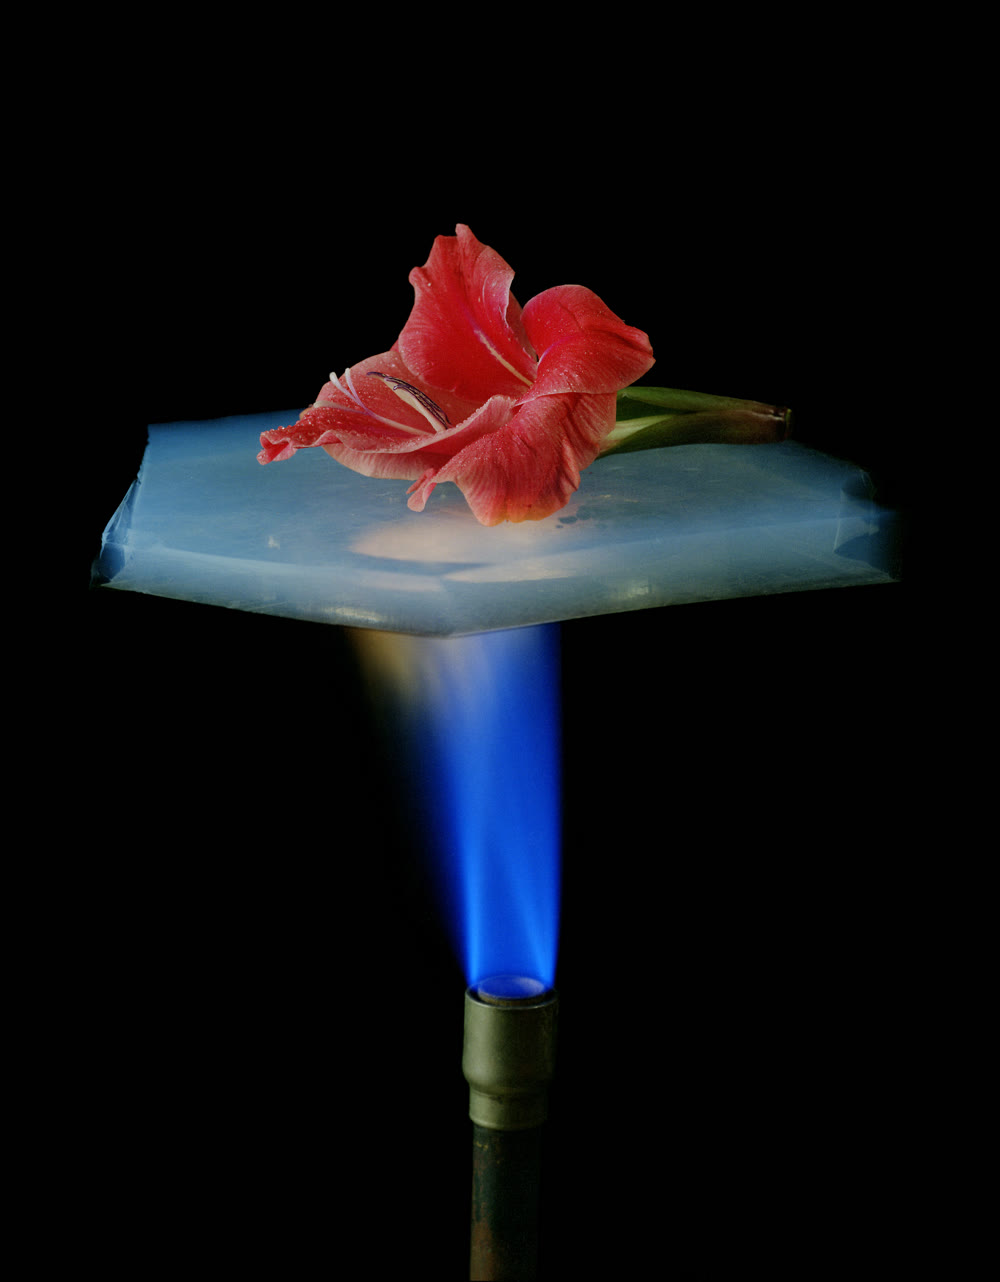
\includegraphics[width=0.38\linewidth]{images/book4/aerogel-flower.jpg}

{\small Een bloem op een plaat \omterm{def:b3:inorganic-materials:sol-gel}{silica-aerogel} boven een gasvlam: de
\omterm{def:b3:inorganic-materials:sol-gel}{aerogel}, een gedroogde \omterm{def:b3:colloids:colloid}{gel} die grotendeels lege ruimte is, geleidt warmte
zeer slecht. Foto: NASA/JPL, publiek domein.}
\end{omfigure}

\section{Syntheseroutes}

\begin{definition}[Keramische methode]\label{def:b3:inorganic-materials:ceramic-method}
De \emph{keramische methode}\index{keramische methode} maakt een vaste
verbinding door de vaste beginstoffen samen te vermalen en ze te
verhitten, vaak dagenlang en met tussentijds opnieuw malen, bij
temperaturen die hoog genoeg zijn opdat ionen door de vaste stoffen
kunnen diffunderen.
\end{definition}

De reactie van twee vaste stoffen vindt plaats op hun contactvlak, en het
product vormt ertussen een laag waar de ionen daarna doorheen moeten: de
traagste stap is de diffusie, en die vertraagt naarmate de laag dikker
wordt.

\begin{proposition}[Parabolische groei]\label{prop:b3:inorganic-materials:parabolic}
Als de groei van een productlaag beperkt wordt door de diffusie erdoorheen,
groeit haar dikte als $x^2 = kt$.
\end{proposition}

\begin{proof}
Met vaste concentraties op de twee vlakken van de laag volgt de flux
erdoorheen de wet van Fick, $J = D\Delta c/x$. De laag groeit evenredig met de flux:
$\dd x/\dd t = \lambda J = \lambda D\Delta c/x$, met $\lambda$ het volume product per getransporteerde mol. Dan is
$x\,\dd x = \lambda D\Delta c\,\dd t$, en integreren vanaf $x = 0$ bij $t = 0$ geeft $x^2 = 2\lambda D\Delta c\,t = kt$.
\end{proof}

Een verdubbeling van de deeltjesgrootte vermenigvuldigt de reactietijd
dus met vier: vandaar het fijn vermalen, het mengen op atomaire schaal in
een precursor (een gemengd oxalaat of een citraatgel die tot het
doelproduct ontleedt), of een route via oplossing.

\begin{definition}[Sol-gelproces]\label{def:b3:inorganic-materials:sol-gel}
Het \emph{sol-gelproces}\index{sol-gelproces} maakt een oxide door
hydrolyse en condensatie van moleculaire precursoren, meestal alkoxiden,
in oplossing: de oplossing wordt een \omterm{def:b3:colloids:colloid}{sol} van kleine oxideclusters, daarna
een \omterm{def:b3:colloids:colloid}{gel}, een continu vast netwerk gevuld met vloeistof. Gedroogd door
verdamping krimpt de \omterm{def:b3:colloids:colloid}{gel} tot een dichte \emph{xerogel}\index{xerogel};
gedroogd boven het kritieke punt van de vloeistof, wat haar verwijdert
zonder grensvlak vloeistof-gas, behoudt hij zijn volume als
\emph{aerogel}\index{aerogel}.
\end{definition}

\begin{omfigure}
\setchemfig{atom sep=2.0em}
\schemestart
\chemfig{RO-Si(-[2]OR)(-[6]OR)-OR}
\+ \chemfig{H_2O}
\arrow{->[hydrolyse]}[,1.4]
\chemfig{RO-Si(-[2]OR)(-[6]OR)-OH}
\+ ROH
\schemestop
\par\bigskip
\schemestart
\chemfig{{\equiv}Si-OH}
\+
\chemfig{HO-Si{\equiv}}
\arrow{->[condensatie]}[,1.6]
\chemfig{{\equiv}Si-O-Si{\equiv}}
\+ \chemfig{H_2O}
\schemestop
\par\medskip

{\small Sol-gelchemie van een siliciumalkoxide (R: een alkylgroep, ethyl
in tetraethylorthosilicaat): water vervangt alkoxygroepen door
hydroxygroepen, en twee silanolen condenseren tot een siloxaanbrug.
Herhaald bouwen de condensaties een driedimensionaal silicanetwerk op.}
\end{omfigure}

Samen geven de twee reacties, voor een volledige reactie,
$\ce{Si(OC2H5)4 + 2H2O -> SiO2 + 4C2H5OH}$. Zure katalyse maakt de hydrolyse snel en de
condensatie traag, wat dunne, ketenachtige polymeren geeft; basische
katalyse het omgekeerde, wat dichte deeltjes geeft. Coatings
(antireflectielagen op glas) worden gemaakt door een onderdeel in de \omterm{def:b3:colloids:colloid}{sol}
te dompelen en het eruit te trekken.

\begin{definition}[Hydrothermale synthese]\label{def:b3:inorganic-materials:hydrothermal}
\emph{Hydrothermale synthese}\index{hydrothermale synthese} kristalliseert
een vaste stof uit water boven zijn normale kookpunt, in een gesloten
vat onder zijn eigen dampdruk;
\emph{solvothermale synthese}\index{solvothermale synthese} doet
hetzelfde in een ander oplosmiddel.
\end{definition}

\begin{definition}[Chemische dampdepositie]\label{def:b3:inorganic-materials:cvd}
\emph{Chemische dampdepositie}\index{chemische dampdepositie} (CVD) laat
een vaste film groeien op een verhit oppervlak door de reactie van
gasvormige precursoren daar, zoals silicium uit silaan, $\ce{SiH4 -> Si + 2H2}$, of diamant uit methaan en waterstof.
\end{definition}

\begin{method}[Een syntheseroute kiezen]\label{met:b3:inorganic-materials:route}
\begin{enumerate}
  \item Een stabiel, vuurvast oxide als bulkpoeder: de \omterm{def:b3:inorganic-materials:ceramic-method}{keramische
        methode}, met een precursor als mengen moeilijk is.
  \item Een metastabiele fase, een fijn poeder of een coating bij lage
        temperatuur: sol-gel of een neerslagreactie.
  \item Grote éénkristallen van een fase die alleen in heet water oplost
        (kwarts) of een raamwerk dat rond een template gebouwd wordt
        (\omterm{def:b3:inorganic-materials:zeolite}{zeolieten}): hydrothermaal.
  \item Een dunne, zuivere film op een substraat (halfgeleiderlagen): CVD.
\end{enumerate}
\end{method}

\begin{inthelab}[Een sol-gelcoating en een autoclaaf]
Tetraethylorthosilicaat wordt geroerd met ethanol, water en een druppel
zuur tot de oplossing helder is; een schoon draagglaasje wordt erin
gedompeld en met een constante lage snelheid eruit getrokken, gedroogd en
verhit, waarna een silicafilm achterblijft die dun genoeg is om
interferentiekleuren te vertonen. Voor een \omterm{def:b3:inorganic-materials:hydrothermal}{hydrothermale synthese} worden
de beginstoffen in een binnenvat van polytetrafluoretheen gebracht, tot
hoogstens ongeveer twee derde gevuld zodat de uitzettende vloeistof het
vat niet vult, afgesloten in een stalen autoclaaf en in een oven verhit;
de autoclaaf wordt pas geopend als hij koud is.
\end{inthelab}

\begin{omfigure}
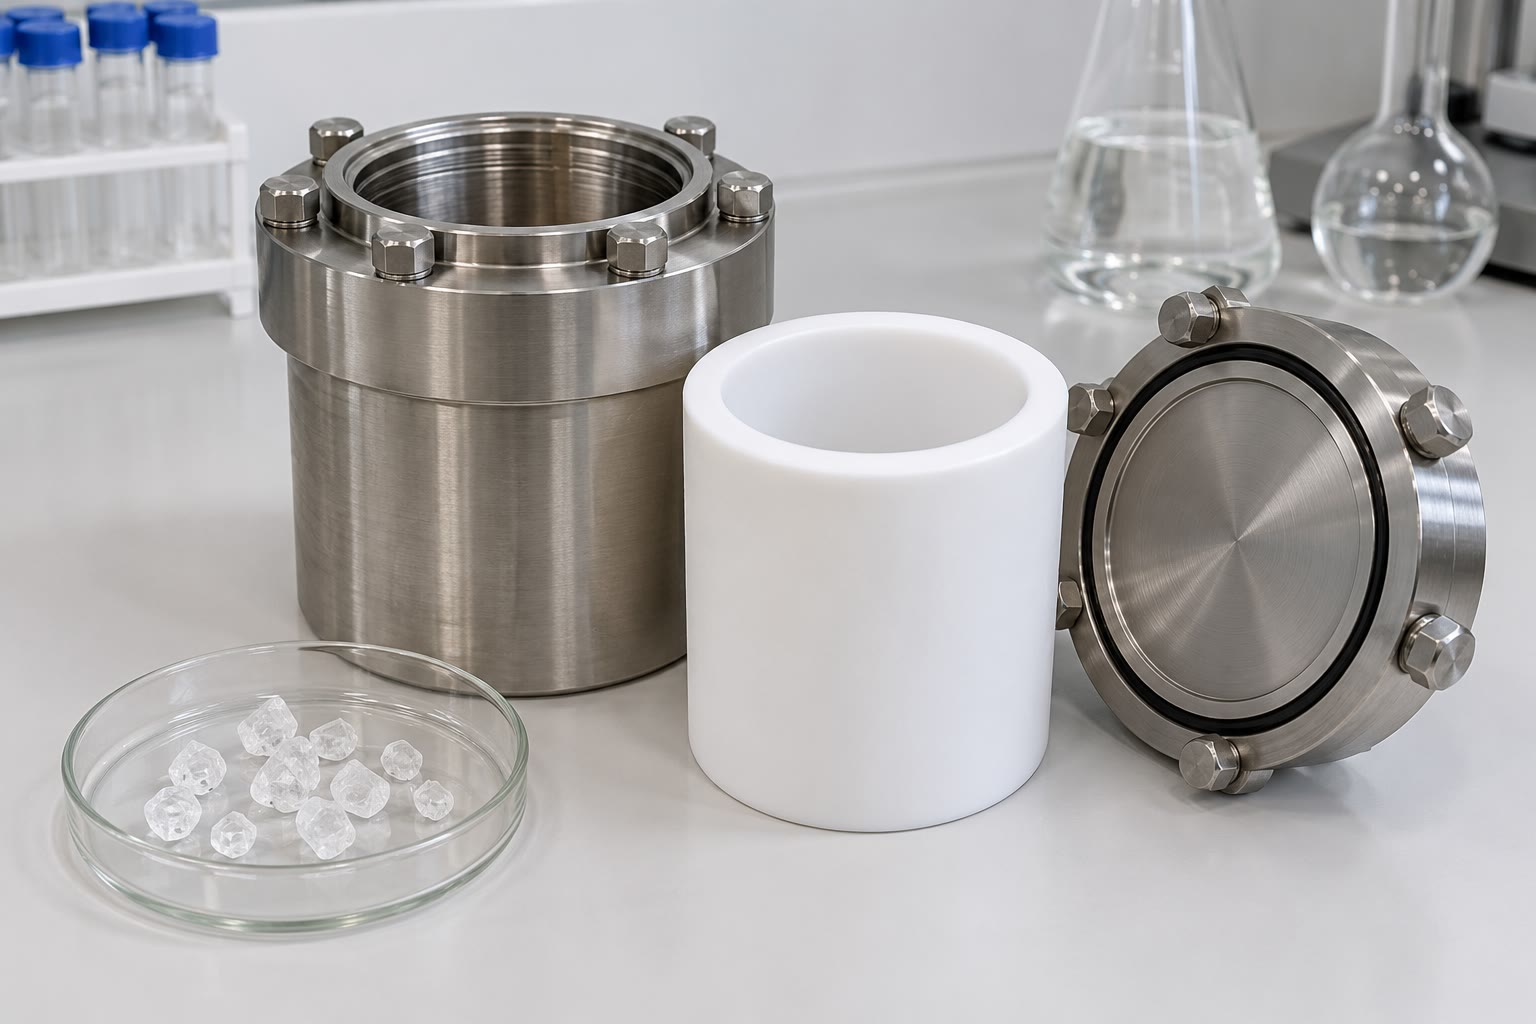
\includegraphics[width=0.5\linewidth]{images/book4/ai/b3-23-autoclave.jpg}

{\small Een laboratoriumautoclaaf voor \omterm{def:b3:inorganic-materials:hydrothermal}{hydrothermale synthese}: een stalen
romp met een vastgeschroefd deksel, een wit polymeren binnenvat dat het
reactiemengsel bevat, en kristallen die erin gegroeid zijn.}
\end{omfigure}

\section{Keramiek en glazen}

\begin{definition}[Keramiek]\label{def:b3:inorganic-materials:ceramic}
\emph{Keramiek}\index{keramiek} is een anorganische, niet-metallische vaste
stof die gemaakt wordt door een poeder te verhitten: oxiden, nitriden en
carbiden, of kleiproducten.
\end{definition}

\begin{definition}[Perovskietstructuur]\label{def:b3:inorganic-materials:perovskite}
De \emph{perovskietstructuur}\index{perovskietstructuur} van een oxide $\mathrm{ABO_3}$
heeft de kleine kationen B in de centra van octaëders $\mathrm{BO_6}$ die hoekpunten delen, en
de grote kationen A in de twaalfgecoördineerde holten ertussen; in de
ideale kubische cel staat B in het centrum, O in de centra van de vlakken
en A op de hoekpunten.
De \emph{tolerantiefactor}\index{tolerantiefactor} meet hoe goed de ionen
passen:
\[
  t = \frac{r_A + r_O}{\sqrt2\,(r_B + r_O)}.
\]
\end{definition}

\begin{omfigure}
\tdplotsetmaincoords{60}{100}
\begin{tikzpicture}[tdplot_main_coords, scale=1.5, font=\small,
  aA/.style={om atom, ball color=green!45!black, minimum size=7.4mm},
  aB/.style={om atom, ball color=black!35, minimum size=4.4mm},
  aOs/.style={om atom, ball color=red!80, minimum size=4.8mm}]
  \pic[transform shape] {omcubeo={2}};
  % atoms back to front for view 60/100 (depth 0.853x + 0.150y + 0.5z)
  \node[aA] at (0,0,0) {};
  \node[aA] at (0,2,0) {};
  \node[aOs] (o1) at (0,1,1) {};
  \node[aA] at (0,0,2) {};
  \node[aOs] (o2) at (1,1,0) {};
  \node[aA] at (0,2,2) {};
  \node[aOs] (o3) at (1,0,1) {};
  \node[aB] (b) at (1,1,1) {};
  \node[aOs] (o4) at (1,2,1) {};
  \node[aA] at (2,0,0) {};
  \node[aOs] (o5) at (1,1,2) {};
  \node[aA] at (2,2,0) {};
  \node[aOs] (o6) at (2,1,1) {};
  \node[aA] at (2,0,2) {};
  \node[aA] at (2,2,2) {};
  \begin{scope}[on background layer]
    \draw[omMeth!70, line width=0.6pt] (o1.center) -- (o2.center) -- (o6.center) -- (o5.center) -- cycle
      (o3.center) -- (o2.center) -- (o4.center) -- (o5.center) -- cycle
      (o1.center) -- (o3.center) -- (o6.center) -- (o4.center) -- cycle;
    \draw[bond] (b.center) -- (o1.center) (b.center) -- (o2.center) (b.center) -- (o3.center)
      (b.center) -- (o4.center) (b.center) -- (o5.center) (b.center) -- (o6.center);
  \end{scope}
  \node[anchor=west] at (2,3.35,2) {A};
  \node[anchor=west] at (2,3.35,1) {O};
  \node[anchor=west] at (2,3.35,0) {B};
  \node[aA, minimum size=4mm] at (2,3.2,2) {};
  \node[aOs, minimum size=3.2mm] at (2,3.2,1) {};
  \node[aB, minimum size=3mm] at (2,3.2,0) {};
\end{tikzpicture}

{\small De kubische perovskietcel $\mathrm{ABO_3}$: een kation B (grijs) in het centrum van een
octaëder van zes oxide-ionen in de centra van de vlakken (groene ribben),
de kationen A op de hoekpunten. Elk ion A op een hoekpunt wordt gedeeld
door acht cellen en elk zuurstofion door twee: één A, één B en drie O per
cel.}
\end{omfigure}

\begin{proposition}[Ideale tolerantiefactor]\label{prop:b3:inorganic-materials:tolerance}
In de ideale kubische perovskiet, waarin de ionen elkaar raken langs de
richtingen B--O en A--O, is $t = 1$.
\end{proposition}

\begin{proof}
Met ribbe $a$ liggen B in het centrum en O in het centrum van een vlak $a/2$ uit elkaar: $r_B + r_O = a/2$.
A op een hoekpunt en O in het centrum van een aangrenzend vlak liggen een
halve vlakdiagonaal uit elkaar: $r_A + r_O = a\sqrt2/2$. Delen geeft $(r_A + r_O)/(r_B + r_O) = \sqrt2$, dus $t = 1$.
\end{proof}

Als $t$ iets kleiner is dan 1, is het ion A te klein voor zijn holte en
kantelen de octaëders om zich eromheen te sluiten, wat de symmetrie
verlaagt; als $t$ groter is dan 1,
is het ion B te klein voor zijn octaëder en kan het uit het centrum
verschuiven.

\begin{definition}[Ferro-elektrische stof]\label{def:b3:inorganic-materials:ferroelectric}
Een \emph{ferro-elektrische stof}\index{ferro-elektrische stof} is een
kristal met een spontane elektrische polarisatie die een aangelegd
elektrisch veld kan omkeren.
\end{definition}

% ledger: rion:Ba2+XII, rion:Ti4+VI, rion:O2-VI
Bariumtitanaat is het klassieke voorbeeld: met $r(\ce{Ba^2+}) = \qty{161}{pm}$ (twaalfgecoördineerd),
$r(\ce{Ti^4+}) = \qty{60.5}{pm}$ en $r(\ce{O^2-}) = \qty{140}{pm}$ is $t = 1.06$. Onder een overgangstemperatuur
verschuiven de titaanionen uit het centrum, allemaal in dezelfde richting
binnen een domein, en raakt het kristal gepolariseerd; de enorme
permittiviteit rond de overgang maakt bariumtitanaat tot het diëlektricum
van de meeste keramische condensatoren.

\begin{definition}[Oxideglazen]\label{def:b3:inorganic-materials:glass}
Een \emph{oxideglas}\index{oxideglas} is een amorfe vaste oxidestof,
gemaakt door een smelt af te koelen zonder kristallisatie. Zijn
\emph{netwerkvormers}\index{netwerkvormer} ($\ce{SiO2}$, $\ce{B2O3}$, $\ce{P2O5}$) bouwen een continu netwerk van
veelvlakken die hoekpunten delen; zijn
\emph{netwerkwijzigers}\index{netwerkwijziger}
($\ce{Na2O}$, $\ce{CaO}$) verbreken bruggen in dat netwerk, waarbij elk toegevoegd oxide-ion
één overbruggend zuurstofatoom omzet in twee niet-overbruggende, met de
kationen in de holten.
\end{definition}

\begin{omfigure}
\begin{tikzpicture}
\begin{axis}[name=c, width=0.5\linewidth, axis equal image, hide axis, xmin=-1.2, xmax=12.6, ymin=-1.2, ymax=8.7]
\addplot[quiver={u=\thisrow{u}, v=\thisrow{v}}, -, black!60, line width=0.6pt] table {figdata/out/bachelor-3-glass-network-crystal-bonds.dat};
\addplot[only marks, mark=*, mark size=2.2pt, omDef] table {figdata/out/bachelor-3-glass-network-crystal-T.dat};
\addplot[only marks, mark=*, mark size=1.3pt, omThm, mark options={fill=white}] table {figdata/out/bachelor-3-glass-network-crystal-O.dat};
\end{axis}
\begin{axis}[at={(c.east)}, anchor=west, xshift=0.2cm, width=0.5\linewidth, axis equal image, hide axis, xmin=-1.2, xmax=12.6, ymin=-1.2, ymax=8.7]
\addplot[quiver={u=\thisrow{u}, v=\thisrow{v}}, -, black!60, line width=0.6pt] table {figdata/out/bachelor-3-glass-network-glass-bonds.dat};
\addplot[only marks, mark=*, mark size=2.2pt, omDef] table {figdata/out/bachelor-3-glass-network-glass-T.dat};
\addplot[only marks, mark=*, mark size=1.3pt, omThm, mark options={fill=white}] table {figdata/out/bachelor-3-glass-network-glass-O.dat};
\addplot[only marks, mark=*, mark size=1.5pt, omThm] table {figdata/out/bachelor-3-glass-network-glass-NBO.dat};
\addplot[only marks, mark=*, mark size=2.6pt, omProp] table {figdata/out/bachelor-3-glass-network-glass-Na.dat};
\end{axis}
\end{tikzpicture}

{\small Een tweedimensionaal beeld van een kristal en een glas met
dezelfde samenstelling (blauw: drievoudig gecoördineerde vormers; open
rode cirkels: overbruggende zuurstofatomen). Links herhaalt het kristal
één ring. Rechts het glas: elke vormer heeft nog drie zuurstofatomen op
bijna dezelfde afstanden, maar de ringen hebben vijf, zes of zeven
leden en niets herhaalt zich; op twee plaatsen heeft een wijziger een
brug verbroken, wat twee niet-overbruggende zuurstofatomen (gevuld rood)
en een kation (oranje) in de holte achterlaat. Modelnetwerk, ontspannen
met veren.}
\end{omfigure}

William Zachariasen stelde in 1932 dat een oxide gemakkelijk een glas
vormt als zijn kation omringd is door weinig zuurstofatomen (drie of
vier), elk zuurstofatoom hoogstens twee kationen verbindt, en de
veelvlakken hoekpunten delen en geen ribben of vlakken: dan kost een
willekeurig netwerk weinig meer energie dan het kristal. Vensterglas is
silica met natrium- en calciumoxide als wijzigers, die de smelttemperatuur
verlagen. Gehard afdekglas voor telefoons wordt in gesmolten
kaliumnitraat gedrenkt: grotere ionen $\ce{K+}$ vervangen ionen $\ce{Na+}$ in het oppervlak en zetten het,
omdat ze krap zitten, onder druk, zodat barsten zich niet openen.

\section{Poreuze vaste stoffen: zeolieten en raamwerken}

\begin{definition}[Zeolieten]\label{def:b3:inorganic-materials:zeolite}
Een \emph{zeoliet}\index{zeoliet} is een kristallijn aluminosilicaat
waarvan het raamwerk van tetraëders $\ce{SiO4}$ en $\ce{AlO4}$ die hoekpunten delen, kooien en
kanalen van moleculaire grootte insluit, met uitwisselbare kationen en
water erin. Een
\emph{moleculaire zeef}\index{moleculaire zeef} is een poreuze vaste stof
die moleculen toelaat volgens hun grootte;
\emph{vormselectiviteit}\index{vormselectiviteit} is de sturing van een
reactie door de grootte en de vorm van de poriën waarin ze plaatsvindt.
\end{definition}

Elke tetraëder $\ce{AlO4}$ draagt één negatieve lading meer dan een $\ce{SiO4}$
(aluminium(III) in plaats van silicium(IV)); kationen in de kooien, $\ce{Na+}$ of $\ce{Ca^2+}$,
compenseren haar en kunnen uitgewisseld worden.

\begin{proposition}[Regel van Löwenstein]\label{prop:b3:inorganic-materials:lowenstein}
In een zeolietraamwerk delen twee tetraëders $\ce{AlO4}$ nooit een zuurstofatoom: verbindingen Al--O--Al
ontbreken (een waarneming aan alle bekende aluminosilicaatraamwerken).
Daaruit volgt dat de verhouding Si/Al van een \omterm{def:b3:inorganic-materials:zeolite}{zeoliet} minstens 1 is.
\end{proposition}

\begin{proof}[Bewijs van het gevolg]
Elk aluminiumatoom heeft vier zuurstofatomen, die volgens de regel elk
met een siliciumatoom gedeeld worden:
$4N_{\mathrm{Al}}$ verbindingen Al--O--Si. Elk siliciumatoom heeft maar vier zuurstofatomen, zodat het deelneemt aan
hoogstens vier zulke verbindingen: $4N_{\mathrm{Al}} \le 4N_{\mathrm{Si}}$, d.w.z.\ $N_{\mathrm{Si}}/N_{\mathrm{Al}} \ge 1$. Gelijkheid dwingt elk
siliciumatoom vier aluminiumburen te hebben: Si en Al wisselen elkaar af.
\end{proof}

\begin{omfigure}
\tdplotsetmaincoords{55}{135}
\begin{tikzpicture}[tdplot_main_coords, scale=0.85, font=\small, baseline=(current bounding box.center),
  tSi/.style={circle, inner sep=0pt, minimum size=2.6mm, draw=black!70, fill=omDef!80},
  tAl/.style={circle, inner sep=0pt, minimum size=2.6mm, draw=black!70, fill=omProp!80}]
  % edges of a truncated octahedron (vertices: permutations of (0, +-1, +-2));
  % hidden edges (both faces facing away for this view) dashed
  \foreach \a/\b/\c/\d/\e/\f in {-2/-1/0/-2/0/-1, -2/-1/0/-2/0/1, -2/-1/0/-1/-2/0, -2/0/-1/-2/1/0, -2/0/-1/-1/0/-2, -1/-2/0/0/-2/-1, -1/-2/0/0/-2/1, -1/0/-2/0/-1/-2, -1/0/-2/0/1/-2, 0/-2/-1/0/-1/-2, 0/-2/-1/1/-2/0, 0/-1/-2/1/0/-2}
    \draw[black!40, dashed] (\a,\b,\c) -- (\d,\e,\f);
  \foreach \a/\b/\c/\d/\e/\f in {-2/0/1/-2/1/0, -2/0/1/-1/0/2, -2/1/0/-1/2/0, -1/0/2/0/-1/2, -1/0/2/0/1/2, -1/2/0/0/2/-1, -1/2/0/0/2/1, 0/-2/1/0/-1/2, 0/-2/1/1/-2/0, 0/-1/2/1/0/2, 0/1/-2/0/2/-1, 0/1/-2/1/0/-2, 0/1/2/0/2/1, 0/1/2/1/0/2, 0/2/-1/1/2/0, 0/2/1/1/2/0, 1/-2/0/2/-1/0, 1/0/-2/2/0/-1, 1/0/2/2/0/1, 1/2/0/2/1/0, 2/-1/0/2/0/-1, 2/-1/0/2/0/1, 2/0/-1/2/1/0, 2/0/1/2/1/0}
    \draw[black!75, line width=0.7pt] (\a,\b,\c) -- (\d,\e,\f);
  % T atoms back to front; hidden ones paler
  \foreach \x/\y/\z/\k/\v in {-2/-1/0/Si/0, -1/-2/0/Al/0, -2/0/-1/Al/0, 0/-2/-1/Si/0, -1/0/-2/Si/0, 0/-1/-2/Al/0, -2/0/1/Al/1, 0/-2/1/Si/1, -2/1/0/Si/1, 1/-2/0/Al/1, 0/1/-2/Al/1, 1/0/-2/Si/1, -1/0/2/Si/1, 0/-1/2/Al/1, -1/2/0/Al/1, 2/-1/0/Si/1, 0/2/-1/Si/1, 2/0/-1/Al/1, 0/1/2/Al/1, 1/0/2/Si/1, 0/2/1/Si/1, 2/0/1/Al/1, 1/2/0/Al/1, 2/1/0/Si/1}
    \node[t\k, opacity=0.35+0.65*\v] at (\x,\y,\z) {};
\end{tikzpicture}
\hspace{1.2cm}
\begin{tikzpicture}[font=\small, scale=0.8, baseline=(current bounding box.center)]
  \foreach \i in {0,1,2} \foreach \j in {0,1,2} {
    \fill[omDef!70] ($(2.2*\i,2.2*\j)+(-0.28,-0.28)$) rectangle +(0.56,0.56);
  }
  \foreach \i in {0,1} \foreach \j in {0,1,2} {
    \draw[black!70, line width=0.8pt] (2.2*\i+0.28,2.2*\j) -- (2.2*\i+0.75,2.2*\j);
    \draw[black!70, line width=0.8pt] (2.2*\i+1.45,2.2*\j) -- (2.2*\i+1.92,2.2*\j);
    \node[draw=black!70, regular polygon, regular polygon sides=6, minimum size=5.6mm, inner sep=0pt] at (2.2*\i+1.1,2.2*\j) {};
  }
  \foreach \i in {0,1,2} \foreach \j in {0,1} {
    \draw[black!70, line width=0.8pt] (2.2*\i,2.2*\j+0.28) -- (2.2*\i,2.2*\j+0.75);
    \draw[black!70, line width=0.8pt] (2.2*\i,2.2*\j+1.45) -- (2.2*\i,2.2*\j+1.92);
    \node[draw=black!70, regular polygon, regular polygon sides=6, minimum size=5.6mm, inner sep=0pt] at (2.2*\i,2.2*\j+1.1) {};
  }
  \node[font=\scriptsize, align=center] at (1.1,-0.85) {$\ce{Zn4O}$-knoop $+$ tereftalaatlinker};
\end{tikzpicture}

{\small Links: een sodalietkooi, de bouweenheid van \omterm{def:b3:inorganic-materials:zeolite}{zeoliet} A, met een
tetraëdrisch atoom op elk hoekpunt (de zuurstofatomen, in het midden van
elke ribbe, zijn niet getekend); silicium (blauw) en aluminium (oranje)
wisselen elkaar af, zoals de regel van Löwenstein vereist als Si/Al = 1. Rechts: een laag van een
\omterm{def:b3:inorganic-materials:mof}{metaal-organisch raamwerk}, schematisch: clusters $\ce{Zn4O}$ (vierkanten), verbonden door
linkers van benzeen-1,4-dicarboxylaat (ringen) tot een kubisch rooster
met grote poriën.}
\end{omfigure}

\begin{method}[Formule en uitwisselingscapaciteit van een zeoliet]\label{met:b3:inorganic-materials:zeolite-formula}
\begin{enumerate}
  \item Schrijf het raamwerk als $\mathrm{[(AlO_2)_x(SiO_2)_y]^{x-}}$: Si/Al $= y/x$.
  \item De lading van het raamwerk $-x$ wordt gecompenseerd door kationen: $x$ eenwaardige of $x/2$
        tweewaardige.
  \item De uitwisselingscapaciteit is de hoeveelheid uitwisselbare lading
        per gram:
        $x/M$ mol eenwaardige kationen, $x/2M$ mol tweewaardige, met $M$ de
        molaire massa van de formule zoals ze gewogen wordt (watervrij
        of gehydrateerd).
\end{enumerate}
\end{method}

\begin{proposition}[Uitwisselingscapaciteit]\label{prop:b3:inorganic-materials:exchange-capacity}
De capaciteit van een \omterm{def:b3:inorganic-materials:zeolite}{zeoliet} voor een kation met lading $z$ is $x/(zM)$ mol per gram,
waarin $x$ het aantal aluminiumatomen is in een formule met molaire massa $M$.
\end{proposition}

\begin{proof}
Elk aluminiumatoom draagt één negatieve lading bij aan het raamwerk; de
elektrische neutraliteit vereist $x$ eenheden positieve lading, allemaal uitwisselbaar, dus
$x/z$ kationen met lading $z$ per formule-eenheid, d.w.z.\ per massa $M$.
\end{proof}

% ledger: iza:LTA.window, iza:MFI.channels
\omterm{def:b3:inorganic-materials:zeolite}{Zeoliet} A heeft vensters van acht tetraëders, \qty{0.41}{nm} breed: water
en kleine ionen gaan erdoor, vertakte moleculen niet. ZSM-5 heeft twee
stelsels kanalen van tien tetraëders, ongeveer 0.51 tot
\qty{0.56}{nm}: bij de omzetting van methanol of de alkylering van
tolueen diffundeert het slanke \textit{para}-xyleen veel sneller naar buiten dan
zijn isomeren \textit{ortho} en \textit{meta}, die achterblijven en isomeriseren. Dat is
\omterm{def:b3:inorganic-materials:zeolite}{vormselectiviteit}.

\begin{definition}[Metaal-organische raamwerken]\label{def:b3:inorganic-materials:mof}
Een \emph{metaal-organisch raamwerk}\index{metaal-organisch raamwerk} (MOF)
is een kristallijne vaste stof, opgebouwd uit metaalionen of -clusters
die door polytope organische linkers tot een poreus netwerk verbonden
zijn. Een \emph{secundaire bouweenheid}\index{secundaire bouweenheid} is
de metaalcluster met zijn coördinerende groepen, behandeld als één knoop
van het net; \emph{reticulaire synthese}\index{reticulaire synthese} is
het ontwerpen van een raamwerk door knopen en linkers met een gegeven
geometrie te kiezen zodat ze zich tot een gekozen net assembleren.
\end{definition}

% ledger: cod:MOF5.formula, cod:MOF5.a
In MOF-5 zijn clusters $\ce{Zn4O}$ met zes carboxylaatgroepen octaëdrische knopen,
en linkers van benzeen-1,4-dicarboxylaat verbinden ze langs de ribben van
een kubisch net, $a = \qty{25.82}{\angstrom}$ voor een cel van acht knopen. De linker vervangen door een
langere behoudt het net en vergroot de poriën: dat is het reticulaire
idee. Zulke raamwerken hebben specifieke oppervlakken van duizenden
vierkante meter per gram en worden onderzocht voor de opslag van
waterstof en methaan en het afvangen van koolstofdioxide.

\begin{definition}[Poriegrootten]\label{def:b3:inorganic-materials:pores}
% ledger: pore:micro, pore:macro
Volgens afspraak zijn \emph{microporiën}\index{microporie} smaller dan
\qty{2}{nm},
\emph{mesoporiën}\index{mesoporie} tussen 2 en \qty{50}{nm}, en
\emph{macroporiën}\index{macroporie} breder dan \qty{50}{nm}.
\end{definition}

\omterm{def:b3:inorganic-materials:zeolite}{Zeolieten} en de meeste MOF's zijn microporeus; silicagels en \omterm{def:b3:inorganic-materials:sol-gel}{aerogels}
mesoporeus.

\section{Nanodeeltjes}

\begin{definition}[Nanomaterialen]\label{def:b3:inorganic-materials:nano}
Een \emph{nanomateriaal}\index{nanomateriaal} heeft minstens één
afmeting tussen ongeveer 1 en \qty{100}{nm}; een
\emph{nanodeeltje}\index{nanodeeltje} heeft er alle
drie.
\end{definition}

\begin{proposition}[Magische clusters]\label{prop:b3:inorganic-materials:magic}
Een cuboctaëdrische cluster uit een centraal atoom en $n$ volledige schillen bevat
\[
  N(n) = \frac{10n^3 + 15n^2 + 11n + 3}{3}
\]
atomen, waarvan er $10n^2 + 2$ aan het oppervlak liggen: 13, 55, 147, 309, \dots
\end{proposition}

\begin{proof}
De $k$-de schil van een cuboctaëder heeft 12 hoekpunten, 24 ribben met elk $k - 1$ atomen
erin, 8 driehoekige vlakken met elk $(k - 1)(k - 2)/2$ inwendige atomen en 6
vierkante vlakken met $(k - 1)^2$: in totaal $12 + 24(k - 1) + 4(k - 1)(k - 2) + 6(k - 1)^2 = 10k^2 + 2$. Dan is
$N(n) = 1 + \sum_{k=1}^{n}(10k^2 + 2) = 1 + \frac{10n(n + 1)(2n + 1)}{6} + 2n$, wat uitgewerkt de formule geeft; de
buitenste schil, $10n^2 + 2$ atomen, is het oppervlak.
\end{proof}

\begin{omfigure}
\begin{tikzpicture}
\begin{axis}[name=a, width=0.47\linewidth, height=5.4cm, xmin=0, xmax=18, ymin=0, ymax=1,
  axis lines=left, xlabel={diameter / \unit{nm}}, ylabel={fractie atomen aan het oppervlak},
  tick label style={font=\scriptsize}, label style={font=\small}]
\addplot[omDef, thick, mark=*, mark size=1pt] table[x=diam_nm, y=fsurf] {figdata/out/bachelor-3-nanoparticle-size.dat};
\end{axis}
\begin{axis}[at={(a.east)}, anchor=west, xshift=1.5cm, width=0.47\linewidth, height=5.4cm,
  xmin=0.8, xmax=6, ymin=0, ymax=3, axis lines=left,
  xlabel={straal $R$ / \unit{nm}}, ylabel={opsluitingsenergie / \unit{eV}},
  tick label style={font=\scriptsize}, label style={font=\small}]
\addplot[omThm, thick] table[x=R_nm, y=dE_eV] {figdata/out/bachelor-3-nanoparticle-size-b.dat};
\end{axis}
\end{tikzpicture}

{\small Links: fractie atomen aan het oppervlak van cuboctaëdrische
goudclusters tegen hun diameter: meer dan de helft bij clusters kleiner
dan ongeveer
\qty{3}{nm}, nog een vijfde bij \qty{8}{nm}. Rechts: opsluitingsenergie
van een elektron-gatpaar in een bolvormige \omterm{def:b3:inorganic-materials:quantum-dot}{kwantumdot} (model met
\omterm{def:b3:quantum-model-systems:oscillator}{gereduceerde massa} $0.10\,m_e$),
die bij de \omterm{def:b3:solid-state:band}{bandkloof} opgeteld wordt en daalt als $1/R^2$.}
\end{omfigure}

Met een groot deel van zijn atomen aan het oppervlak, waar ze minder
buren hebben, smelt een \omterm{def:b3:inorganic-materials:nano}{nanodeeltje} bij een lagere temperatuur dan het
bulkmetaal, is het reactiever, en kan het een veel betere katalysator
zijn: bulkgoud is inert, gouddeeltjes van enkele nanometer oxideren
koolstofmonoxide bij kamertemperatuur.

\begin{definition}[Kwantumdots]\label{def:b3:inorganic-materials:quantum-dot}
Een \emph{kwantumdot}\index{kwantumdot} is een nanokristal van een
\omterm{def:b3:solid-state:classes}{halfgeleider} dat klein genoeg is opdat de opsluiting van zijn elektronen
en \omterm{def:b3:solid-state:carriers}{gaten} zijn \omterm{def:b3:solid-state:band}{bandkloof} boven die van de bulkvaste stof verhoogt.
\end{definition}

\begin{theorem}[Opsluiting in een bol]\label{thm:b3:inorganic-materials:quantum-dot}
Een deeltje met massa $m$, door oneindige wanden opgesloten in een bol met straal $R$, heeft
de grondtoestandsenergie $E = \hbar^2\pi^2/(2mR^2) = h^2/(8mR^2)$, met golffunctie $\psi \propto \sin(\pi r/R)/r$.
\end{theorem}

\begin{proof}
Voor een bolsymmetrische toestand $\psi(r) = u(r)/r$ geeft de laplaciaan
$\nabla^2\psi = u''/r$, zodat de \omterm{thm:b3:quantum-model-systems:schrodinger}{schrödingervergelijking} binnenin $-\frac{\hbar^2}{2m}u'' = Eu$ wordt, die van een deeltje op een
lijn. De oplossing met $\psi$ eindig in het centrum heeft $u(0) = 0$: $u = \sin(kr)$, met $E = \hbar^2k^2/2m$.
De wand vereist $u(R) = 0$, dus $kR = \pi$ voor de grondtoestand, en $E = \hbar^2\pi^2/(2mR^2)$.
\end{proof}

In een dot zijn het elektron en het \omterm{def:b3:solid-state:carriers}{gat} allebei opgesloten; de energie van
de laagste aanslag is in eerste benadering $E_g + h^2/(8\mu R^2)$, met $\mu$ hun \omterm{def:b3:quantum-model-systems:oscillator}{gereduceerde
massa} (hun coulombaantrekking verlaagt haar een beetje). De straal
halveren vermenigvuldigt de opsluitingsenergie met vier:
cadmiumselenidedots van enkele nanometer gloeien rood, groen of blauw,
alleen naargelang hun grootte, en worden als emitters in beeldschermen
gebruikt.

\begin{definition}[Oppervlakteplasmonresonantie]\label{def:b3:inorganic-materials:plasmon}
Een \emph{oppervlakteplasmonresonantie}\index{oppervlakteplasmonresonantie}
is een collectieve oscillatie van de geleidingselektronen van een
metaalnanodeeltje, aangedreven door licht; ze geeft een sterke
absorptieband waarvan de golflengte afhangt van het metaal, de grootte en
de vorm van het deeltje en zijn omgeving.
\end{definition}

Gouden \omterm{def:b3:inorganic-materials:nano}{nanodeeltjes} van enkele tientallen nanometer absorberen groen
licht en zien er in een glas of een \omterm{def:b3:colloids:colloid}{colloïd} robijnrood uit; als ze
aggregeren, verschuift de band naar langere golflengten en wordt de kleur
blauw: de basis van veel sneltests, waarin een met antilichamen bekleed
goudcolloïd zich tot een gekleurde lijn verzamelt.

\section{Koolstofnanomaterialen}

\begin{definition}[Koolstofnanomaterialen]\label{def:b3:inorganic-materials:carbon}
Een \emph{fullereen}\index{fullereen} is een gesloten kooimolecuul van
koolstofatomen, elk gebonden aan drie andere, met vijf- en zesringen,
zoals het icosaëdrische $\ce{C60}$. Een \emph{koolstofnanobuis}\index{koolstofnanobuis} is een vel
grafiet dat opgerold is tot een naadloze cilinder van ongeveer een
nanometer breed.
\emph{Grafeen}\index{grafeen} is één enkele laag grafiet, één atoom dik.
\end{definition}

\begin{proposition}[Twaalf vijfhoeken]\label{prop:b3:inorganic-materials:euler}
Elk \omterm{def:b3:inorganic-materials:carbon}{fullereen} heeft precies twaalf vijfhoeken, wat zijn aantal zeshoeken
ook is.
\end{proposition}

\begin{proof}
Een gesloten kooi is een veelvlak: de formule van Euler $V - E + F = 2$ geldt. Elk atoom heeft
drie bindingen en elke binding twee atomen: $2E = 3V$. Met $p$ vijfhoeken en $h$ zeshoeken
geeft het tellen van de ribben via de vlakken $2E = 5p + 6h$, en $F = p + h$. Dan is $V = 2E/3$ en luidt de
formule van Euler $-E/3 + p + h = 2$, d.w.z.\ $-(5p + 6h)/6 + p + h = 2$, dus $p/6 = 2$: $p = 12$.
\end{proof}

\begin{omfigure}
\begin{tikzpicture}[scale=0.62, font=\small]
  \def\hexd{0.6}
  \begin{scope}
    \clip (-0.4,-0.5) rectangle (9.6,5.2);
    \foreach \i in {-3,...,10} \foreach \j in {-1,...,6} {
      \pgfmathsetmacro\cx{1.7320508*\hexd*(\i + 0.5*\j)}
      \pgfmathsetmacro\cy{1.5*\hexd*\j}
      \draw[black!45] ({\cx+\hexd*cos(30)},{\cy+\hexd*sin(30)})
        \foreach \k in {90,150,...,390} { -- ({\cx+\hexd*cos(\k)},{\cy+\hexd*sin(\k)}) };
    }
  \end{scope}
  \draw[->, thick, omDef] (0,0) -- ({1.7320508*\hexd},0) node[below right, font=\scriptsize, fill=white, inner sep=1pt] {$\mathbf a_1$};
  \draw[->, thick, omDef] (0,0) -- ({1.7320508*\hexd*0.5},{1.5*\hexd}) node[left, font=\scriptsize, fill=white, inner sep=1pt] {$\mathbf a_2$};
  \draw[->, very thick, omThm] (0,0) -- ({1.7320508*\hexd*(4+0.5*2)},{1.5*\hexd*2}) node[above right, font=\scriptsize, fill=white, inner sep=1pt] {$\mathbf C_h = 4\mathbf a_1 + 2\mathbf a_2$};
  \draw[dashed, omMeth, thick] (0,0) -- ({1.7320508*\hexd*9},0) node[right, font=\scriptsize] {zigzag $(n, 0)$};
  \draw[dashed, omProp, thick] (0,0) -- ({1.7320508*\hexd*5*1.5},{1.5*\hexd*5}) node[below right, font=\scriptsize, fill=white, inner sep=1pt] {armstoel $(n, n)$};
\end{tikzpicture}

{\small Een grafeenvel en de chirale vector van een nanobuis: het vel zo
oprollen dat de punt van $\mathbf C_h = n\mathbf a_1 + m\mathbf a_2$ zijn oorsprong raakt, geeft de buis $(n, m)$, hier $(4, 2)$.
Langs $\mathbf a_1$ is de rand van een buis $(n, 0)$ een zigzag; langs $\mathbf a_1 + \mathbf a_2$, onder 30°, is die van een buis $(n, n)$
een armstoel.}
\end{omfigure}

\begin{proposition}[Metallische en halfgeleidende nanobuizen]\label{prop:b3:inorganic-materials:nanotube}
Een enkelwandige \omterm{def:b3:inorganic-materials:carbon}{koolstofnanobuis} $(n, m)$ is metallisch als $n - m$ een veelvoud van 3 is, en
anders een \omterm{def:b3:solid-state:classes}{halfgeleider}. \admitted
\end{proposition}

Een derde van alle mogelijke buizen is dus metallisch, waaronder elke
armstoelbuis; de kloof van de andere daalt naarmate hun diameter groeit.
\omterm{def:b3:inorganic-materials:carbon}{Grafeen} zelf heeft helemaal geen kloof: zijn \omterm{def:b3:solid-state:band}{valentieband} en zijn
\omterm{def:b3:solid-state:band}{geleidingsband} raken elkaar in afzonderlijke punten, en zijn elektronen
bewegen alsof ze geen massa hadden.

\begin{safety}{\ghs[0.62cm]{GHS02}\ghs[0.62cm]{GHS07}\ghs[0.62cm]{GHS08}}
% ledger: ghs4:TEOS
Tetraethylorthosilicaat: ontvlambare vloeistof en damp, schadelijk bij
inademing, irriterend voor de ogen en de luchtwegen; gehanteerd in een
zuurkast. Nanopoeders: de fijnste deeltjes dringen diep in de longen
door, en veel ervan zijn nog niet ingedeeld; ze worden afgewogen en
gehanteerd in een omkasting of als suspensie, nooit als los stof in de
open lucht.
\end{safety}

\begin{omfigure}
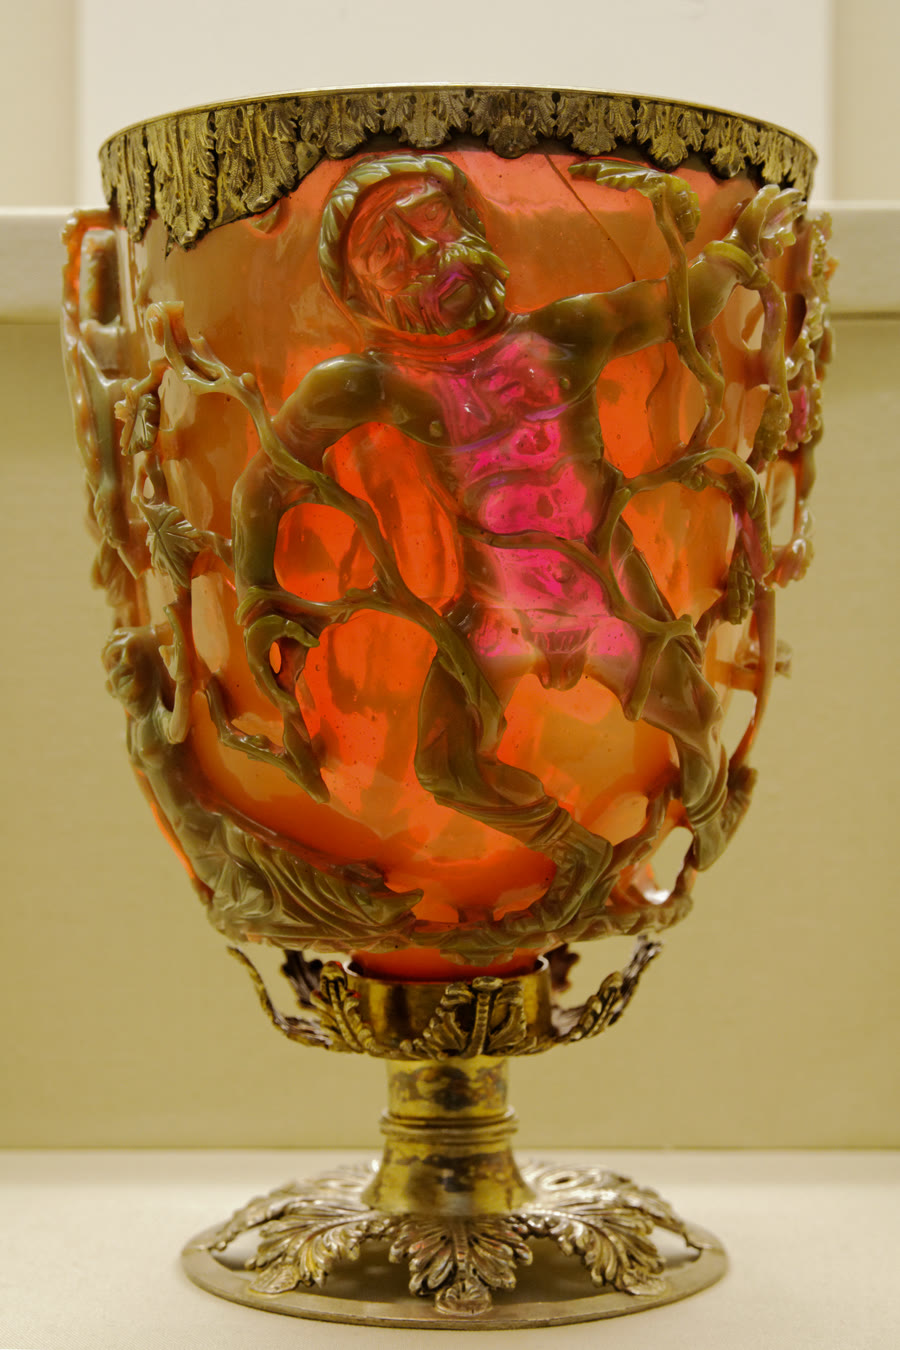
\includegraphics[width=0.32\linewidth]{images/book4/lycurgus-cup.jpg}

{\small De Lycurgusbeker, een Romeins glas uit de vierde eeuw, van
binnenuit belicht: in teruggekaatst licht ziet hij er groen uit en in
doorvallend licht rood, een effect van goud-zilvernanodeeltjes in het
glas. Foto: Marie-Lan Nguyen, CC BY
2.5.}
\end{omfigure}

\begin{history}[Nanodeeltjes vóór het woord, en een voetbal van koolstof]
Glasmakers kleurden glas rood met goud lang voordat iemand wist waarom;
de Lycurgusbeker toont het effect op zijn opvallendst. Michael Faraday
maakte in de jaren 1850 goudcolloïden en zag dat hun kleur kwam van
deeltjes die te klein waren om te zien. In 1985 ontdekten Harold Kroto,
Robert Curl en Richard Smalley, die grafiet met een laser verdampten, dat
clusters van zestig koolstofatomen uitzonderlijk stabiel waren, en
stelden ze de gesloten kooi van twaalf vijfhoeken en twintig zeshoeken
voor; ze ontvingen de Nobelprijs voor de Scheikunde van 1996.
\end{history}

\section{Oefeningen}

\begin{exercise}[$\star$]\label{exo:b3:inorganic-materials:1}
Een productlaag tussen twee vaste stoffen is na \qty{10}{h} \qty{2.0}{\micro\metre} dik. Hoe lang duurt het tot ze
\qty{6.0}{\micro\metre} dik is, als de groei parabolisch is?
\end{exercise}

\begin{exercise}[$\star$]\label{exo:b3:inorganic-materials:2}
Schrijf de hydrolyse van tetraethylorthosilicaat tot kiezelzuur op, de
condensatie van twee moleculen kiezelzuur, en de totaalreactie die
silica geeft.
\end{exercise}

\begin{exercise}[$\star$]\label{exo:b3:inorganic-materials:3}
Deel $\ce{SiO2}$, $\ce{B2O3}$, $\ce{Na2O}$ en $\ce{CaO}$ in als \omterm{def:b3:inorganic-materials:glass}{netwerkvormers} of -wijzigers, en zeg wat
$\ce{Na2O}$ met het netwerk van silica doet.
\end{exercise}

\begin{exercise}[$\star$]\label{exo:b3:inorganic-materials:4}
Hoeveel vijfhoeken en zeshoeken heeft $\ce{C70}$? Hoeveel bindingen?
\end{exercise}

\begin{exercise}[$\star\star$]\label{exo:b3:inorganic-materials:5}
% ledger: rion:Sr2+XII, rion:Ca2+XII, rion:Ba2+XII, rion:Ti4+VI, rion:O2-VI
Bereken de \omterm{def:b3:inorganic-materials:perovskite}{tolerantiefactoren} van $\ce{SrTiO3}$, $\ce{BaTiO3}$ en $\ce{CaTiO3}$ met de twaalfgecoördineerde stralen
van $\ce{Sr^2+}$ (\qty{144}{pm}), $\ce{Ba^2+}$ (\qty{161}{pm}) en $\ce{Ca^2+}$ (\qty{134}{pm}), $r(\ce{Ti^4+}) = \qty{60.5}{pm}$ en $r(\ce{O^2-}) = \qty{140}{pm}$. Wat
voorspellen ze?
\end{exercise}

\begin{exercise}[$\star\star$]\label{exo:b3:inorganic-materials:6}
Een \omterm{def:b3:inorganic-materials:zeolite}{zeoliet} X heeft de watervrije formule $\mathrm{Na_{86}[(AlO_2)_{86}(SiO_2)_{106}]}$ (gegevens van de oefening).
Geef Si/Al en zijn uitwisselingscapaciteit voor $\ce{Ca^2+}$ in millimol per gram.
\end{exercise}

\begin{exercise}[$\star\star$]\label{exo:b3:inorganic-materials:7}
% ledger: lat:Au
Goud is kubisch vlakgecentreerd met $a = \qty{407.8}{pm}$. Schat het aantal schillen van een
cuboctaëdrisch gouddeeltje van ongeveer \qty{5}{nm} breed, zijn aantal
atomen en de fractie aan zijn oppervlak.
\end{exercise}

\begin{exercise}[$\star\star$]\label{exo:b3:inorganic-materials:8}
Een \omterm{def:b3:solid-state:classes}{halfgeleider} heeft een bulkkloof van \qty{1.74}{eV}, en zijn elektron en \omterm{def:b3:solid-state:carriers}{gat} een \omterm{def:b3:quantum-model-systems:oscillator}{gereduceerde
massa} van $0.10\,m_e$ (gegevens van de oefening). Schat de kleur van het licht dat uitgezonden wordt door
dots met een straal van 2.0 en \qty{3.0}{nm}, met verwaarlozing van de
coulombaantrekking.
\end{exercise}

\begin{exercise}[$\star\star$]\label{exo:b3:inorganic-materials:9}
Zijn de nanobuizen $(10, 10)$, $(10, 0)$, $(9, 0)$ en $(12, 8)$ metallisch of halfgeleidend? Welke
zijn armstoelbuizen, welke zigzagbuizen?
\end{exercise}

\begin{exercise}[$\star\star\star$]\label{exo:b3:inorganic-materials:10}
% ledger: cod:MOF5.formula, cod:MOF5.a, cod:MOF5.Z
MOF-5, $\mathrm{Zn_4O(C_8H_4O_4)_3}$, is kubisch met $a = \qty{25.82}{\angstrom}$ en acht formule-eenheden per cel.
Bereken zijn dichtheid. Als één gram een oppervlak van $\qty{3000}{m^2}$ heeft (gegevens van de
oefening), hoeveel voetbalvelden van $\qty{105}{m} \times \qty{68}{m}$ is dat?
\end{exercise}

\begin{exercise}[$\star\star\star$]\label{exo:b3:inorganic-materials:11}
Toon met de schillentelling van \cref{prop:b3:inorganic-materials:magic}
aan dat de oppervlaktefractie van een cuboctaëdrische cluster naar $3/n$ gaat voor grote $n$, en
vergelijk met de exacte fractie voor $n = 8$.
\end{exercise}

\begin{exercise}[$\star\star\star$]\label{exo:b3:inorganic-materials:12}
Een gesloten koolstofkooi met drie bindingen per atoom bevat $p$ vijfhoeken, $h$ zeshoeken
en $s$ zevenhoeken. Toon aan dat $p - s = 12$.
\end{exercise}

\section{Probleem: water ontharden met zeoliet A}

\begin{problem}[{Weekendprobleem --- water ontharden met zeoliet A: de
formule en de regel van Löwenstein, de theoretische
uitwisselingscapaciteit, de zeoliet die voor één wasbeurt nodig is, en
het venster dat calcium binnenlaat en detergenten buitenhoudt}]
\label{pb:b3:inorganic-materials:1}
% ledger: iza:LTA.formula, iza:LTA.window, aw:Na, aw:Al, aw:Si, aw:O, aw:H, aw:Ca, aw:C, rion:Ca2+VI
\omterm{def:b3:inorganic-materials:zeolite}{Zeoliet} A, dat in wasmiddelen gebruikt wordt in plaats van fosfaten, heeft de formule
$\mathrm{Na_{12}[(AlO_2)_{12}(SiO_2)_{12}]\cdot 27H_2O}$ en vensters van \qty{0.41}{nm} breed. Een leidingwater bevat
\qty{2.0}{mmol/L} $\ce{Ca^2+}$, en een wasbeurt gebruikt er \qty{15}{L} van; in de tijd van een wasbeurt bereikt de \omterm{def:b3:inorganic-materials:zeolite}{zeoliet}
60\,\% van zijn capaciteit (gegevens van het probleem).

\medskip\noindent\textbf{Deel I --- De formule.}
\begin{enumerate}
  \item Bereken de molaire massa van de watervrije formule.
  \item Bereken die van de gehydrateerde formule.
  \item Geef Si/Al.
  \item Formuleer de regel van Löwenstein en wat hij hier betekent voor de
        rangschikking van
        Si en Al.
  \item Wat is de lading van het raamwerk per formule?
  \item Bereken de massafractie water in de gehydrateerde \omterm{def:b3:inorganic-materials:zeolite}{zeoliet}.
\end{enumerate}

\medskip\noindent\textbf{Deel II --- Uitwisselingscapaciteit.}
\begin{enumerate}[resume]
  \item Schrijf het uitwisselingsevenwicht op tussen de natriumzeoliet en
        calciumionen.
  \item Hoeveel $\ce{Ca^2+}$ kan één formule opnemen?
  \item Bereken de theoretische capaciteit van de watervrije \omterm{def:b3:inorganic-materials:zeolite}{zeoliet} in mmol $\ce{Ca^2+}$
        per gram.
  \item Bereken haar voor de gehydrateerde \omterm{def:b3:inorganic-materials:zeolite}{zeoliet}.
  \item Druk de watervrije capaciteit uit in milligram $\ce{CaCO3}$ per gram, de gebruikelijke
        eenheid voor waterhardheid.
\end{enumerate}

\medskip\noindent\textbf{Deel III --- Eén wasbeurt.}
\begin{enumerate}[resume]
  \item Bereken de hoeveelheid $\ce{Ca^2+}$ in het water van één wasbeurt.
  \item Bereken de massa gehydrateerde \omterm{def:b3:inorganic-materials:zeolite}{zeoliet} die nodig is bij de
        theoretische capaciteit.
  \item Bereken haar bij 60\,\% van de capaciteit.
  \item Bereken de massa natrium die in het water vrijkomt.
  \item Waarom hebben wasmiddelfabrikanten de fosfaten vervangen?
  \item Waarom neemt \omterm{def:b3:inorganic-materials:zeolite}{zeoliet} A $\ce{Mg^2+}$ trager op dan $\ce{Ca^2+}$?
\end{enumerate}

\medskip\noindent\textbf{Deel IV --- Het venster.}
\begin{enumerate}[resume]
  \item Vergelijk het venster met de diameter van een ion $\ce{Ca^2+}$ (zesgecoördineerde straal
        \qty{100}{pm}).
  \item Wat moet een gehydrateerd ion $\ce{Ca^2+}$ doen om erdoor te gaan?
  \item Waarom blijft een anion van een \omterm{def:b3:colloids:surfactant}{oppervlakteactieve stof}, zoals
        dodecylsulfaat, buiten?
  \item Wat doet \omterm{def:b3:inorganic-materials:zeolite}{zeoliet} A als droogmiddel, en waarom noemt men het een
        \omterm{def:b3:inorganic-materials:zeolite}{moleculaire zeef}?
  \item Hoe zou het vervangen van $\ce{Na+}$ door $\ce{K+}$ de grootte van de toegelaten moleculen veranderen?
  \item Waarom verlaat \textit{para}-xyleen in ZSM-5 de poriën sneller dan \textit{ortho}-xyleen?
  \item Formuleer het resultaat: de theoretische uitwisselingscapaciteit
        van watervrij \omterm{def:b3:inorganic-materials:zeolite}{zeoliet} A
        voor $\ce{Ca^2+}$.
\end{enumerate}
\end{problem}
